\section{Precompilation Instructions and Macros}
\label{sec:macro}
\begin{frame}<beamer>
    \frametitle{Outline}
    \tableofcontents[currentsection]
\end{frame}
\begin{frame}{Precompilation: the Concept (1)}
\begin{itemize}
	\item {It happens before we compile codes to binary}
	\item {Preprocess the codes}
	\item {There are instrustions we use to communicate with the compiler}
\end{itemize}

\begin{figure}
	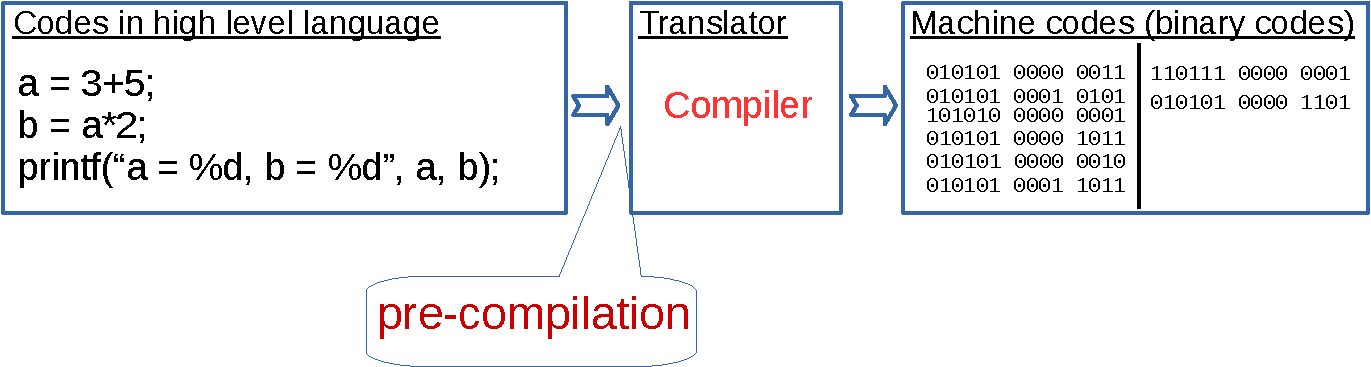
\includegraphics[width=0.9\linewidth]{figs/compil1.pdf}
\end{figure}

\begin{itemize}
	\item {They are executed before compilation is undertaken}
\end{itemize}

\end{frame}

\begin{frame}{Precompilation: the Concept (2)}
\begin{figure}
	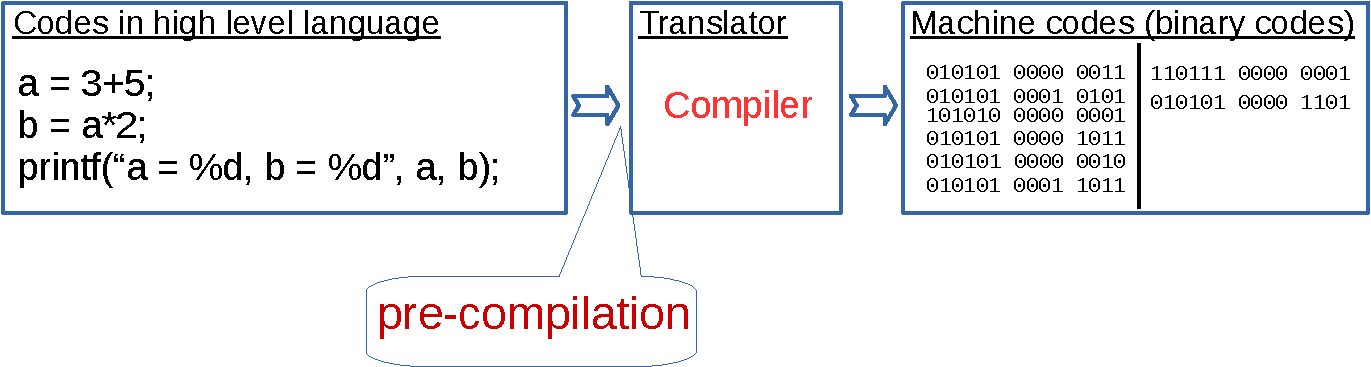
\includegraphics[width=0.9\linewidth]{figs/compil1.pdf}
\end{figure}

\begin{itemize}
	\item {There are instrustions we use to communicate with the compiler}
	\item {They all start with ``\textcolor{red}{\#}'', pronounced as ``sharp''}
	\begin{enumerate}
		\item {\#\textcolor{blue}{include} header file or full path of file}
		\item {\#\textcolor{blue}{define} MACRO}
		\item {\#\textcolor{blue}{if}...\#\textcolor{blue}{else} or \#\textcolor{blue}{if}...\#\textcolor{blue}{else if} MACRO}
		\item {\#\textcolor{blue}{ifndef} MACRO}
		\item {\#\textcolor{blue}{endif}}
	\end{enumerate}
\end{itemize}

\end{frame}

\begin{frame}[fragile]{Precompilation instruction: \#\textcolor{blue}{include} (1)}
\begin{itemize}
	\item {It tells the compiler following thing}
	\begin{enumerate}
		\item {A header file is required to compile the code}
		\item {In the header file, the function that is called in the code is declared}
		\item {Where the compiler is able to find the file}
	\end{enumerate}
\end{itemize}
\begin{columns}
\begin{column}{0.45\linewidth}
\begin{lstlisting}
#include <stdio.h>

\end{lstlisting}
\end{column}
\begin{column}{0.45\linewidth}
\begin{lstlisting}
#include "myfunc.h"

\end{lstlisting}
\end{column}
\end{columns}
\begin{itemize}
	\item {$<$stdio.h$>$ tells the compiler to search in the system default path}
	\item {"myfunc.h" tells the compiler to \textcolor{red}{1}. search in the directed path, \textcolor{red}{2}. then go to system default path}
\end{itemize}
\end{frame}

\begin{frame}[fragile]{Precompilation instruction: \#\textcolor{blue}{include} (2)}
\begin{columns}
\begin{column}{0.52\linewidth}
[myfunc.h]
\begin{lstlisting}[linewidth=0.95\linewidth]
float mypow(float base, int n)
{
   float r = 1;
   int i = 0;
   
   if(n == 0)
   rerturn r;
   
   for(i = 1; i <= n; i++)
   {
      r = base*r;
   }
   return r;
}
\end{lstlisting}
\end{column}
\begin{column}{0.46\linewidth}
[main.c]
\begin{lstlisting}
#include "myfunc.h"
#include <stdio.h>
int main()
{
  float r = mypow(3.14, 3);
  printf("r = %f\n", r);
  return 0;
}
\end{lstlisting}
\end{column}
\end{columns}
\end{frame}

\begin{frame}[fragile]{Instruction for Macros: \#\textcolor{blue}{define} (1)}
\begin{itemize}
	\item {\#\textcolor{blue}{define} allows user to define constants or functions}
	\item {These constants and functions can be later called in the code}
	\item {As a convention, we CAPITALIZE everything}
	\item {However, it is possible that PI is defined elsewhere}
\end{itemize}

\begin{columns}
\begin{column}{0.44\linewidth}
\begin{lstlisting}[xleftmargin=0.02\linewidth]
#define PI 3.1415926
#include <stdio.h>
int main()
{
  float a = 0, r = 4.5;
  a = PI*r*r;
  printf("a = %f\n", a);
  return 0;
}
\end{lstlisting}
\end{column}
\begin{column}{0.14\linewidth}
\begin{center}
\vspace{0.6in}
$\Longrightarrow$
\end{center}
\end{column}
\begin{column}{0.41\linewidth}
\begin{block}{After pre-compilation}
\end{block}
\begin{lstlisting}
#define PI 3.1415926
#include <stdio.h>
int main()
{
  float a = 0, r = 4.5;
  a = 3.1415926*r*r;
  printf("a = %f\n", a);
  return 0;
}
\end{lstlisting}
\end{column}
\end{columns}
\end{frame}

\begin{frame}[fragile]{Instruction for Macros: \#\textcolor{blue}{define} (2)}
\begin{itemize}
	\item {However, it is possible that PI is defined elsewhere}
\end{itemize}

\begin{columns}
\begin{column}{0.44\linewidth}
\begin{lstlisting}
#define PI 3.1415926
#include <stdio.h>
int main()
{
  float a = 0, r = 4.5;
  a = PI*r*r;
  printf("a = %f\n", a);
  return 0;
}
\end{lstlisting}
\end{column}
\begin{column}{0.44\linewidth}
\begin{lstlisting}
#ifndef PI
#define PI 3.1415926
#endif
#include <stdio.h>
int main()
{
  float a = 0, r = 4.5;
  a = PI*r*r;
  printf("a = %f\n", a);
  return 0;
}
\end{lstlisting}
\end{column}
\end{columns}
\end{frame}

\begin{frame}[fragile]{Instruction for Macros: \#\textcolor{blue}{define} (3)}
\begin{itemize}
	\item {Pay attention that the constant has NO type}
	\item {We can similarly define Macro function}
\end{itemize}
\begin{columns}
\begin{column}{0.40\linewidth}
\begin{lstlisting}
#define MULT(x,y) x*y+y
#include <stdio.h>
int main()
{
  float a = 2, r = 4.5;
  a = MULT(a, r);
  printf("a = %f\n", a);
  return 0;
}
\end{lstlisting}
\end{column}
\begin{column}{0.40\linewidth}
\begin{lstlisting}
#ifndef MULT
#define MULT(x,y) x*y+y
#endif
#include <stdio.h>
int main()
{
  float a = 2, r = 4.5;
  a = MULT(a, r)*4;
  printf("a = %f\n", a);
  return 0;
}
\end{lstlisting}
\end{column}
\end{columns}
\begin{itemize}
	\item {Please work out the output for each ...}
\end{itemize}
\end{frame}

\begin{frame}[fragile]{Instruction for Macros: \#\textcolor{blue}{define} (4)}
\begin{itemize}
	\item {Pay attention that the constant has NO type}
	\item {We can similarly define Macro function}
\end{itemize}
\begin{columns}
\begin{column}{0.44\linewidth}
\begin{lstlisting}[linewidth=0.9\linewidth]
#ifndef MULT
#define MULT(x,y) x*y+y
#endif
#include <stdio.h>
int main()
{
  float a = 2, r = 4.5;
  a = MULT(a, r)*4;
  printf("a = %f\n", a);
  return 0;
}
\end{lstlisting}
\end{column}
\begin{column}{0.1\linewidth}
\begin{center}
\vspace{0.6in}
$\Longrightarrow$
\end{center}
\end{column}
\begin{column}{0.40\linewidth}
\begin{block}{After pre-compilation}
\end{block} 
\begin{lstlisting}
#include <stdio.h>
int main()
{
  float a = 2, r = 4.5;
  a = a*r+r*4;
  printf("a = %f\n", a);
  return 0;
}
\end{lstlisting}
\end{column}
\end{columns}
\begin{itemize}
	\item {It is better to put the bracket on the whole}
\end{itemize}
\end{frame}

\begin{frame}[fragile]{Instruction for Macros: \#\textcolor{blue}{define} (5)}
\begin{itemize}
	\item {Pay attention that the constant has NO type}
	\item {We can similarly define Macro function}
\end{itemize}
\begin{columns}
\begin{column}{0.44\linewidth}
\begin{lstlisting}[xleftmargin=0.05\linewidth]
#ifndef MULT
#define MULT(x,y) (x*y+y)
#endif
#include <stdio.h>
int main()
{
  float a = 2, r = 4.5;
  a = MULT(a, r)*4;
  printf("a = %f\n", a);
  return 0;
}
\end{lstlisting}
\end{column}
\begin{column}{0.14\linewidth}
\begin{center}
\vspace{0.6in}
$\Longrightarrow$
\end{center}
\end{column}
\begin{column}{0.42\linewidth}
\begin{block}{After pre-compilation}
\end{block} 
\begin{lstlisting}
#include <stdio.h>
int main()
{
  float a = 2, r = 4.5;
  a = (a*r+r)*4;
  printf("a = %f\n", a);
  return 0;
}
\end{lstlisting}
\end{column}
\end{columns}
\begin{itemize}
	\item {It is better to put the bracket on the whole}
\end{itemize}
\end{frame}

\begin{frame}[fragile]{Instruction for Macros: \#\textcolor{blue}{define} (6)}
\begin{itemize}
	\item {It is literally replacement all the time}
\end{itemize}
\begin{columns}
\begin{column}{0.42\linewidth}
\begin{lstlisting}
#ifndef HI
#define HI "hello"
#define WD	world
#endif
#include <stdio.h>
int main()
{
  printf("HI");
  printf("\n");
  printf(WD);
  printf("\n");
  printf(HI);
  return 0;
}
\end{lstlisting}
\end{column}
\begin{column}{0.40\linewidth}
[Output]
\begin{lstlisting}
??
??
\end{lstlisting}
\end{column}
\end{columns}
\end{frame}

\begin{frame}[fragile]{Instruction for Macros: \#\textcolor{blue}{define} (7)}
\begin{itemize}
	\item {It is literally replacement all the time}
\end{itemize}
\begin{columns}
\begin{column}{0.46\linewidth}
\begin{lstlisting}
#ifndef HI
#define HI "hello"
#define WD	world
#endif
#include <stdio.h>
int main()
{
  printf("HI");
  printf("\n");
  //printf(WD); //<--mistake
  printf("\n");
  printf(HI);
  return 0;
}
\end{lstlisting}
\end{column}
\begin{column}{0.35\linewidth}

[after comment out \textcolor{blue}{line 10},\\output]
\begin{lstlisting}
HI
hello
\end{lstlisting}
\end{column}
\end{columns}
\end{frame}

\begin{frame}[fragile]{Instruction for Macros: \#\textcolor{blue}{ifdef} (1)}
\begin{itemize}
	\item {We can use Macro to control the compilation}
\end{itemize}
\vspace{-0.1in}
\begin{columns}
\begin{column}{0.48\linewidth}
\begin{lstlisting}
#define DEBUG
#include <stdio.h>
int main()
{
  int i = 0, j = 1;
  for(i = 0; i < 5; i++)
  {
     j = i*2+1;
     #ifdef DEBUG
       printf("j = %f\n", j);
     #endif
  }
  return 0;
}
\end{lstlisting}
\end{column}
\begin{column}{0.48\linewidth}
\begin{lstlisting}
//#define DEBUG
#include <stdio.h>
int main()
{
  int i = 0, j = 1;
  for(i = 0; i < 5; i++)
  {
     j = i*2+1;
     #ifdef DEBUG
       printf("j = %f\n", j);
     #endif
  }
  return 0;
}
\end{lstlisting}
\end{column}
\end{columns}
\vspace{-0.2in}
\begin{itemize}
	\item {The code is compiled inside \#\textcolor{blue}{ifdef} only when ``\textbf{DEBUG}'' is defined}
\end{itemize}
\end{frame}

\begin{frame}[fragile]{Instruction for Macros: \#\textcolor{blue}{ifdef} (2)}
\begin{itemize}
	\item {Codes after pre-compilation}
\end{itemize}
\vspace{-0.1in}
\begin{columns}
\begin{column}{0.52\linewidth}
\begin{lstlisting}[xleftmargin=0.02\linewidth, linewidth=0.9\linewidth]
#define DEBUG
#include <stdio.h>
int main()
{
  int i = 0, j = 1;
  for(i = 0; i < 5; i++)
  {
     j = i*2+1;
     printf("j = %f\n", j);
  }
  return 0;
}
\end{lstlisting}
\end{column}
\begin{column}{0.47\linewidth}
\begin{lstlisting}
//#define DEBUG
#include <stdio.h>
int main()
{
  int i = 0, j = 1;
  for(i = 0; i < 5; i++)
  {
     j = i*2+1;
  }
  return 0;
}
\end{lstlisting}
\end{column}
\end{columns}
\vspace{-0.2in}
\begin{itemize}
	\item {The code is compiled inside \#\textcolor{blue}{ifdef} only when ``\textbf{DEBUG}'' is defined}
\end{itemize}
\end{frame}